\documentclass[12pt]{article}
\usepackage{efbox,graphicx}
\efboxsetup{linecolor=black,linewidth=1pt}
\usepackage[utf8]{inputenc}
\usepackage[english]{babel}
\usepackage{amsmath}
\usepackage{natbib}
\usepackage{graphicx}
\usepackage{hyperref}
\usepackage{caption}
\usepackage{caption,float}
\usepackage[vmargin=3cm,hmargin=3cm]{geometry}

\begin{document}

{\centering

\rule{\textwidth}{1.6pt}\vspace*{-\baselineskip}\vspace*{2pt} 
\rule{\textwidth}{0.4pt}\\[\baselineskip] 
{\LARGE Using Autorank, Missingno and Machine learning algorithm to predict bank deposit from clients }
\rule{\textwidth}{0.4pt}\vspace*{-\baselineskip}\vspace{3.2pt}
\rule{\textwidth}{1.6pt}\\[\baselineskip] 

\vspace{20mm} %5mm vertical space
\scshape % Small caps
CMSC 6950 - Computer Based Research Tools and Applications \\ [\baselineskip]
Term Project \\[\baselineskip] 
6th August, 2020 \\[\baselineskip] 
\vspace{20mm} %5mm vertical space
Submitted by \\[\baselineskip]
{\Large Anne Odeh \par}
\vfill
{\itshape Memorial University of Newfoundland \\ St. John's, Canada.\par} 
}

\newpage

{\centering
  \section*{Abstract}
}
This paper presents how to recreate and build upon the data analysis as well as make modification to the code. The project is focused on how the banking industry can approach different subset of customers to subscribe to a financial product. \\\\

\section{Data Exploration}
\subsection{Introduction}
Machine learning has revolutionized the way we see data today, it is used to extract
knowledge from data. Outside of commercial applications, machine learning has had a
tremendous influence on the way data-driven research is done today. The bank dataset can be used to predict if customers would subscribe to a bank deposit. The data set is based on the direct marketing campaigns of a Portuguese banking institution. These marketing campaigns were based on phone calls. More than one contact to a client was required, to know if the product (bank term deposit) was subscribed by a client or not.
\subsection{Dataset Summary}
This dataset has 17 columns and 11163 rows. Below is a detailed description of each column: 

\begin{itemize}

\item age: the age of group of ban customers
\item	job: type of job (admin., blue collar, entrepreneur, housemaid, management, retired, 'self-employed', 'services', 'student', 'technician', 'unemployed', 'unknown')
\item	marital: marital status (divorced, married, single, unknown; note: divorced means divorced or widowed)
\item	education: (primary, secondary, tertiary, and unknown)
\item	default: has credit in default? (no, yes, unknown)
\item	housing: has housing loan? (no, yes, unknown)
\item	loan: has personal loan? (no, yes, unknown)
\item	balance: Balance of the individual
\item	contact: contact communication type (cellular, telephone)
\item	month: last contact month of year 
\item	day: last contact day of the week 
\item	duration: last contact duration, in seconds (numeric). 
\item	campaign: number of contacts performed during this campaign and for this client 
\item pdays: number of days that passed by after the client was last contacted from a previous campaign 
\item	previous: number of contacts performed before this campaign and for this client 
\item poutcome: outcome of the previous marketing campaign (failure, non-existent, success)
\item	deposit: has the client subscribed a term deposit? (yes or no)
\end{itemize}

\newpage
\subsection{Attributes Types}

\begin{table}[h!]
	\centering
	\begin{tabular}{|c|c|}
			\hline
		\textbf{Attributes}& \textbf{Types}\\
		\hline
			\hline
	age	&numeric\\
		\hline
	job	&categorical\\
		\hline
	marital&	categorical\\
		\hline
	education&	categorical\\
		\hline
	default	&categorical\\
		\hline
	housing	&categorical\\
		\hline
	loan	&categorical\\
		\hline
	contact	&categorical\\
		\hline
	balance	&numeric\\
		\hline
	contact	&unknown\\
		\hline
	month&	categorical\\
		\hline
	day	&numeric\\
	    \hline
	duration&	numeric\\
		\hline
	campaign&	numeric\\
		\hline
	pdays	&numeric\\
		\hline
	previous&	numeric\\
		\hline
	poutcome	&unknown\\
		\hline
	deposit&	categorical\\
		\hline
	\end{tabular}

	\caption{Attributes Types}
\end{table}

\newpage
\section{Implementing different python packages for data analysis}
Banks use marketing campaigns as tools to focus on customer needs and their overall satisfaction strategically. Improving customer experience requires truly understanding your customers and relating to them in ways that they understand. This includes taking a 360-degree view of your banking customer and leveraging the gold mine of data available to you today, including: 
\begin{itemize}

\item Core customer information including contact and location data
\item Additional experiential customer information gathered from all stages of the customer life-cycle.
\item Transaction information including checking, savings and credit card transactions; loan draws and repayments; investment positions and balances. 

\end{itemize}
Banks of every size are drenched with data, but harnessing and leveraging that organizational data for more effective banking operations has always been a challenge. In the current market, it’s more important than ever that you understand customers, products, channels and pricing – all to ensure it is tailored towards product offerings to customers while maximizing the potential revenue.\\\\
Using transaction and core customer information, you can determine the life stages and family dynamics that allow for better product bundling and targeted marketing for your customers.
\newpage
\subsection{Missingno}
Missingno was used for analyzing the dataset to visualize any missing data. It allows for  quick visual summary of the completeness of the dataset.  \href{https://github.com/ResidentMario/missingno}{Click for more information on missingno package.} 

\begin{figure}[!htbp]
	\centering
\efbox{	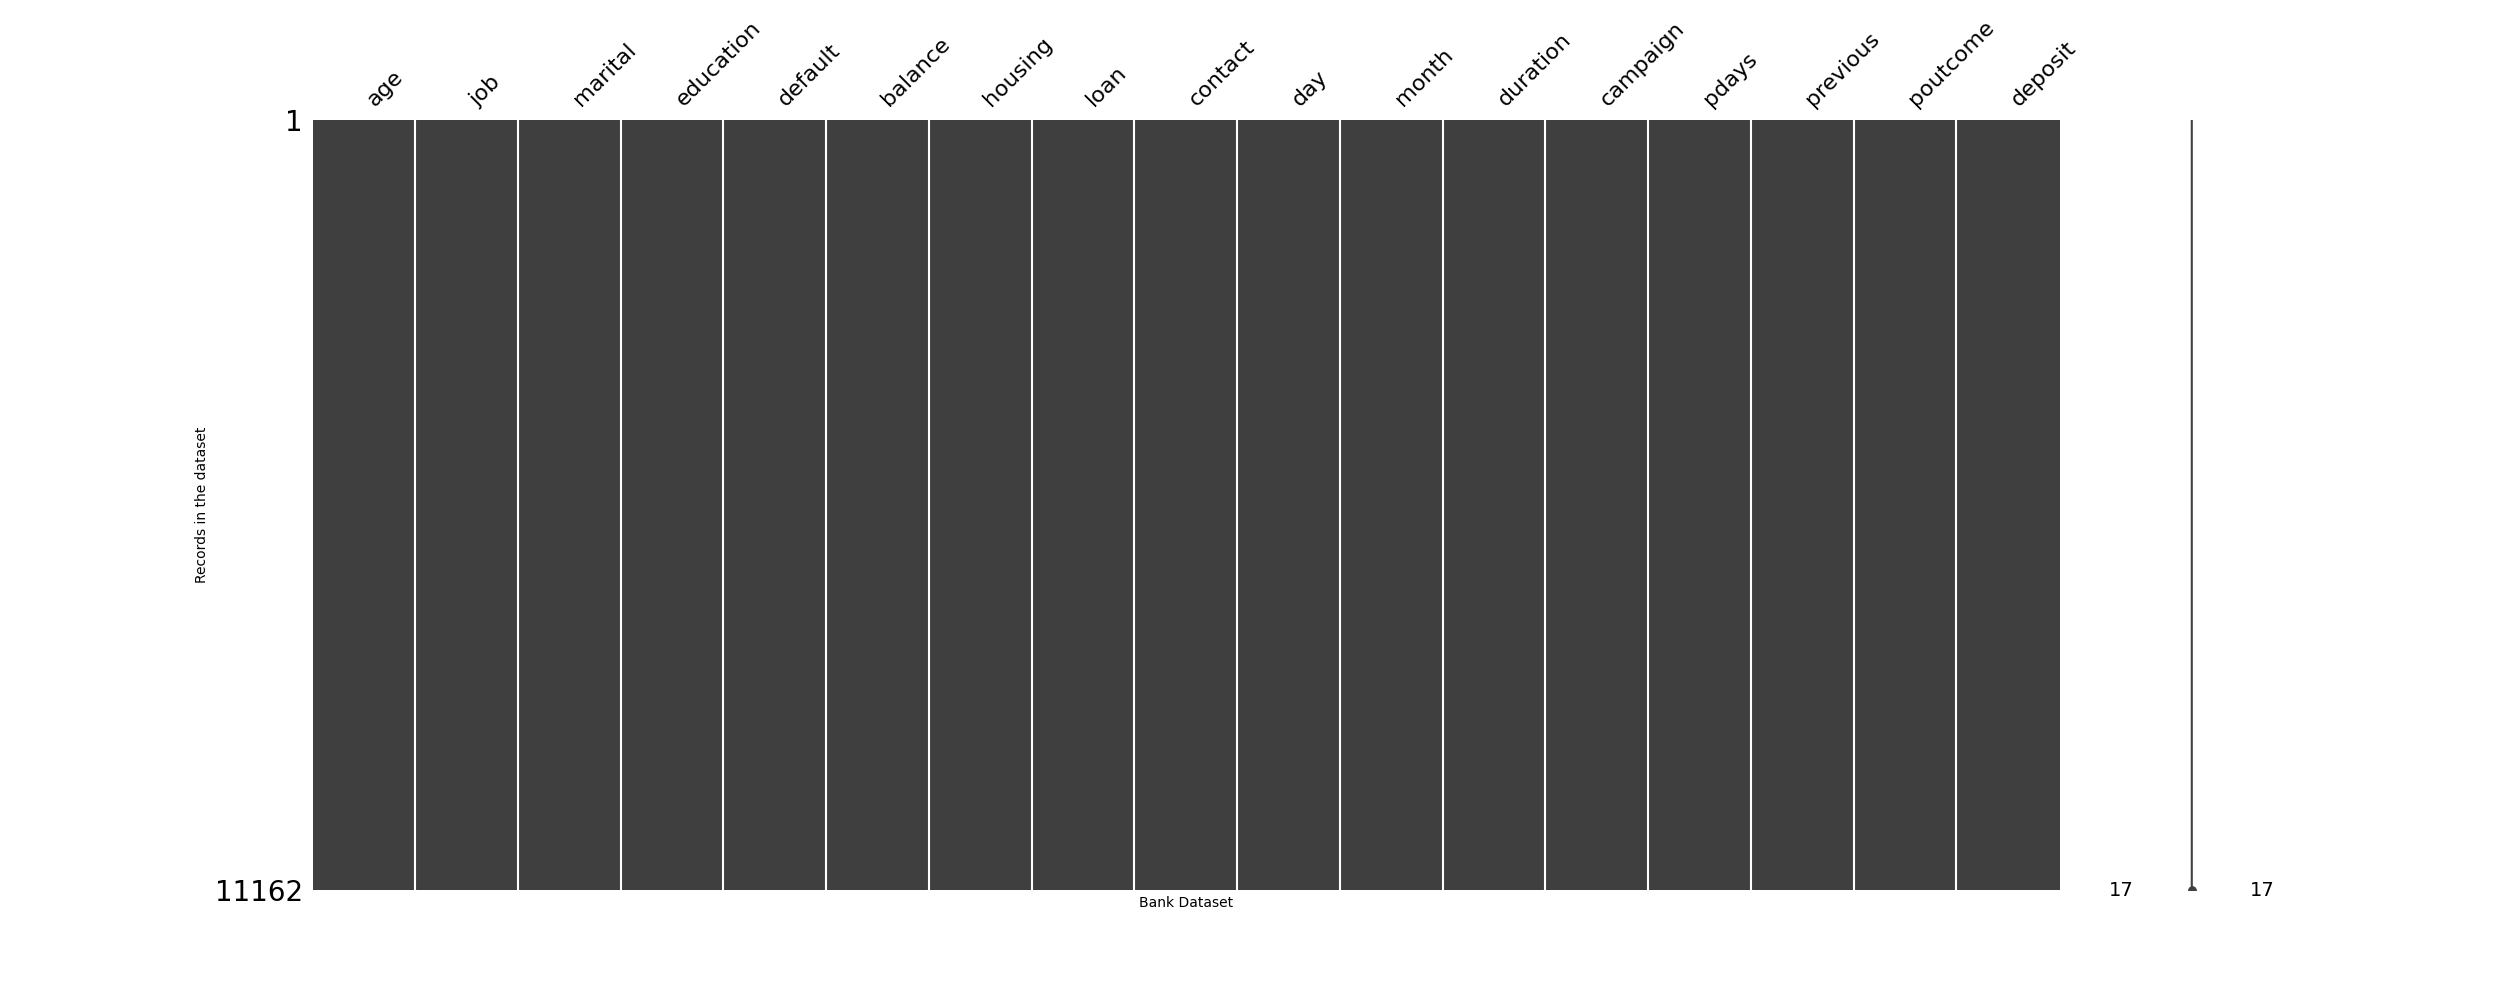
\includegraphics[width=15 cm]{missing_data.png}}
	\caption{Data Completeness}
\end{figure}


\subsection{Autorank}
Autorank was used to achieve a quick statistical analysis of the duration of calls made to different clients with different marital statuses. Banks will find this helpful as it will aid them to design different deposit package that benefits everyone.
 \href{https://pypi.org/project/autorank/#description}{Click for more information on autorank package.} 

\begin{figure}[!htbp]
	\centering
\efbox{	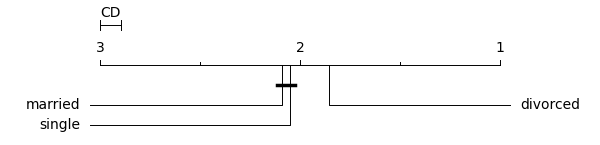
\includegraphics[width=15 cm]{stat_auto_rank.png}}
	\caption{Autorank Plot}
\end{figure}
\newpage
The plot shows the number of contacts with different subset of customers during the campaign.
\begin{figure}[!htbp]
	\centering
	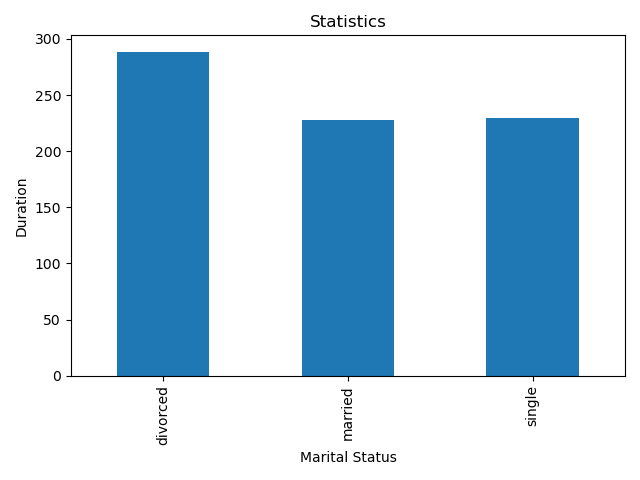
\includegraphics[width=15 cm]{mean.png}
	\caption{Bar Plot of the }
\end{figure}

\newpage
The plot showed that the divorced have considerably low balance. 
\begin{figure}[!htbp]
	\centering
	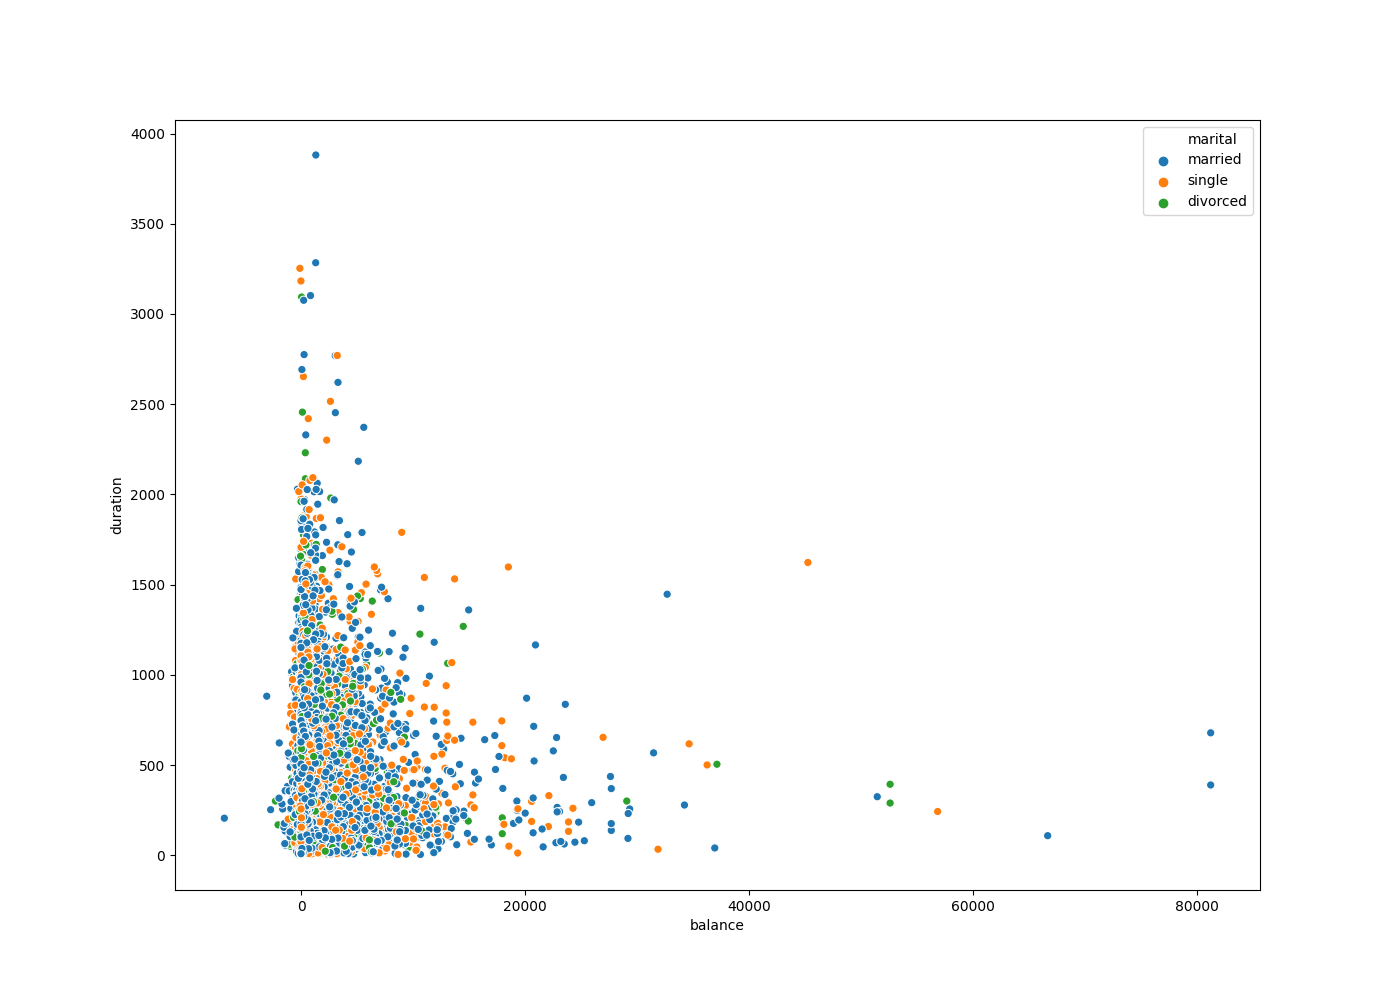
\includegraphics[width=15 cm]{marital_balance.png}
	\caption{Distribution by Marital/Balance}
\end{figure}

\newpage
People who were above the duration status, were more likely to open a term deposit. 78\% of the group that is above average in duration opened term deposits while those that were below average 32\% did not open term deposit accounts. This simply means target individuals who are above average category.
\begin{figure}[!htbp]
	\centering
	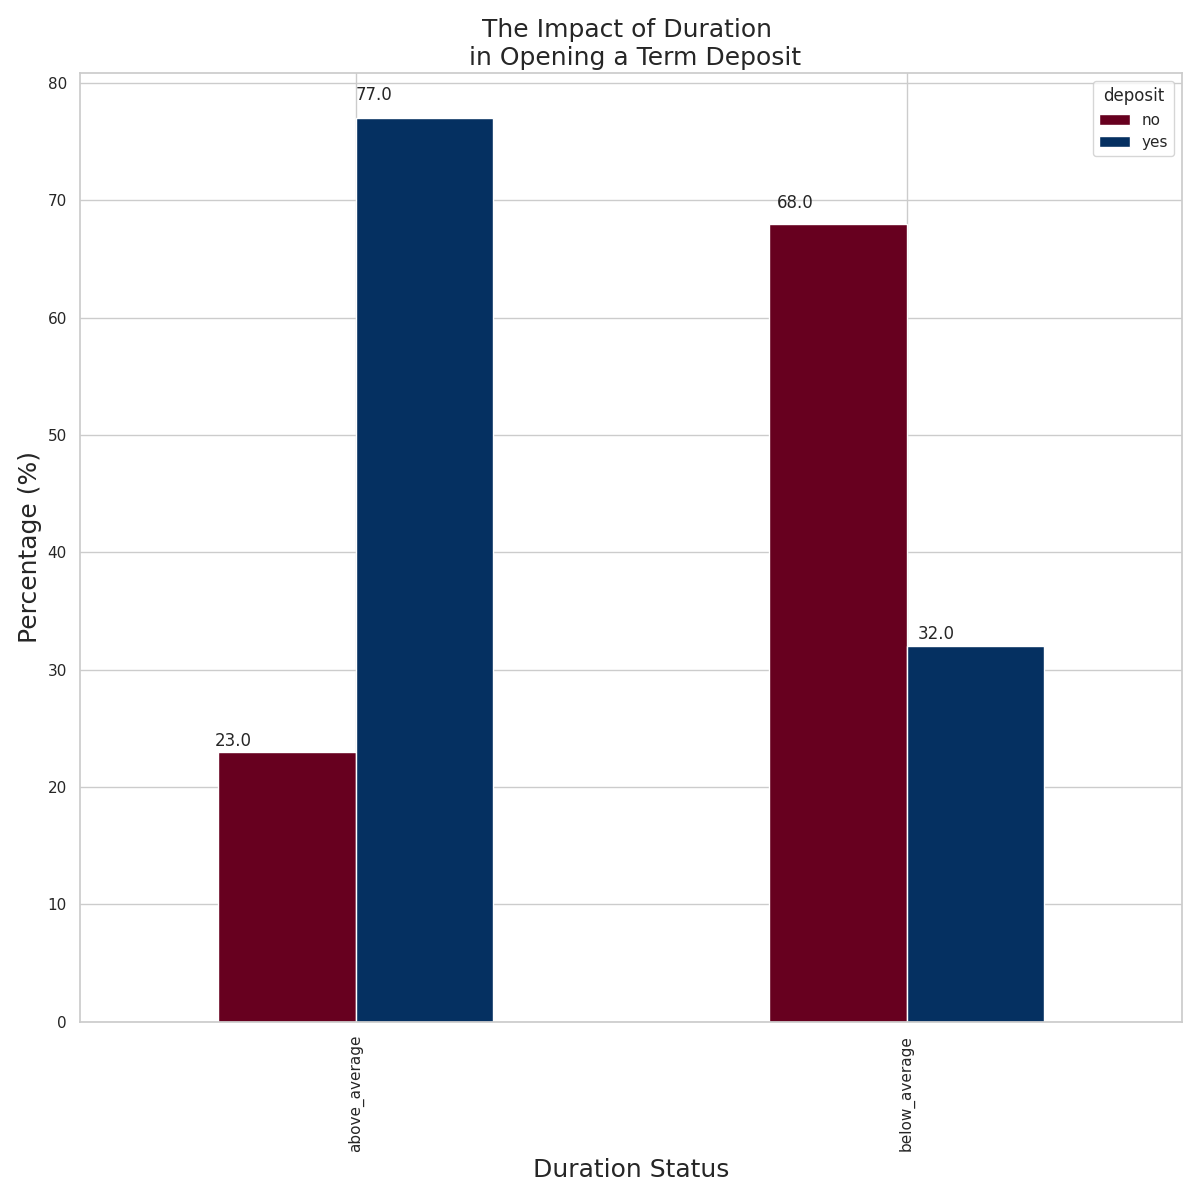
\includegraphics[width=11 cm]{duration.png}
	\caption{Bar Plot of Duration}
\end{figure}

\newpage
\subsection{Using Xgboost to predict campaign outcome}
The beauty of this robust algorithm lies in its scalability, which drives fast learning
through parallel and distributed computing and provides powerful memory use. Xgboost (Extreme Gradient Boosting) is an ensemble learning approach that provides a systematic solution for integrating the multiple learners' predictive capacity.\\\\
Xgboost manages only numeric vectors (0, 1). Therefore, it is imperative to convert
categorical variables to numerical variables by using the method called one-hot encoding. One hot encoding is a process by which categorical variables transform into a type that could be supplied to ML algorithms to do better predictive work (Sundaram, 2020).

The above algorithm was use to model the prediction of the campaign. The accuracy score and testing is 0.912 and 0.850. 

\section{Conclusion}
Overall, Autorank and missingno packages made it easy to perform statistical analysis and visualize any missing data in my dataset. The outcome of the model shows a good predictive score of 0.912. 
\newpage

\begin{thebibliography}{999}

%reference 1
	\bibitem[Martinez, J. (2017)]{ref-software}
	Martinez, J. (2017). Bank Marketing Dataset. Retrieved July 31, 2020, from {\url{https://www.kaggle.com/janiobachmann/bank-marketing-dataset}}

   
%reference 2
	\bibitem[Herbold, S. (2020)]{ref-softwaree}
	S. Herbold (2020). Autorank: A Python package for automated ranking of classifiers. Journal of Open Source Software. https://doi.org/10.21105/joss.02173
	
%reference 3
	\bibitem[S, Moro; P, Cortez ; P, Rita (2014)]{ref-softiwaree}
S. Moro, P. Cortez and P. Rita (2014). A Data-Driven Approach to Predict the Success of Bank Telemarketing. Decision Support Systems, Elsevier, 62:22-31, June 2014

%reference 4
\bibitem[Sundaram, R. (2020)]{ref-ww}
Sundaram, R. (2020). XGBoost Algorithm | XGBoost In Machine Learning. Retrieved 1 August 2020, from https://www.analyticsvidhya.com/blog/2018/09/an-end-to-end-guide-to-understand-the-math-behind-xgboost/


\end{thebibliography}

\end{document}
